\chapter{Results}
We test each variable specified in our methods section over a range of values to examine trends in the reconstruction speed and overall accuracy. Unless otherwise specified, the default values for our simulation are listed in Table \ref{tab:def_vals}. Our error bars are calculated under the assumption of Gaussian noise, and we assume this to be a good approximation of our true noise based on the central limit theorem in statistics.\\

\begin{table}[h]
    \centering
    \begin{tabular}{|c|c|c|c|c|c|c|c|}
    \hline
    Variable: & Precision & Hits (total) & Hits (used) & P-value & $\eta'$-tolerance & $\sigma_{sp}$ & $a$ \\
    \hline
    Value: & single & 5 & 5 & 0.01 & 1.0 & 1 mm & 0.22 \\
    \hline
    \end{tabular}
    \caption{Caption}
    \label{tab:def_vals}
\end{table}

- Each test is run with several basic values that remain unchanged unless otherwise specified: 
- We use 5-hit events, with all 5 hits used in the reconstruction, energy and spatial noise at close to real values (.22 energy noise, 1 mm of spatial noise) and the predicted noise at the same levels
- Each error bar is calculated under the assumption of Gaussian noise, with a p-value of .005
- 

\section{Power}

- We use the WITRN U2 USB Power Monitor to test the power when it's idle and when it's running
- Once plugged in, it displays the average power used and the max power used
- We tested it for a half hour in idle mode - x watts
- We tested it after running our program for 5 minutes - x watts
- We tested it after running for about a half hour - x watts
- This isn't the final hardware, so it probably wouldn't mean much to report the exact values, but the hardware on the APT will be similar, so we expect it to be a good estimate
- draws about 2-4 watts when it's running
- this is well below the 50W we needed to keep under (from Jim), so I think we're good

\section{Precision}
- on a pi, single precision is 32-bit and double precision is 64-bit
- single precision: $3.848x105 \pm 0.513x10^5$ photons/sec vs. double: $5.076x10^5 \pm 0.698x10^5$ photons/sec
- x trials, x photons per trial
- accuracy: 86.12\% vs 86.15\% for accuracy. Not enough that it would make a huge difference for our purposes since our measurements' noise threshold will probably account for a greater error than that.
- since the pi is an in-order processor, it runs comparatively slower with double-precision values than if it were an out-of-order processor
- Using double-precision values reduces rounding error, but it does not give us enough of an increase in accuracy to warrant the reduction in speed.

\section{Parallelism}
- Tested on Cassini because it has more cores
- We run our algorithm on different numbers of cores and calculate the speedup of each trial
- We are using a constant workload for each run, so the speedup in the latency is the sequential execution time divided by the parallel execution time.
- The speedup in throughput is the number of cores used for each run multiplied by the speedup in latency for each run. *** include the equation(s)
- Shows an overall linear trend in speedup, which means that our program has good scalability.

\begin{figure}
    \centering
    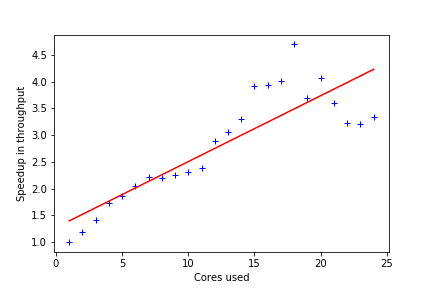
\includegraphics[width=0.7\textwidth]{graphs/Cassini_throughput_speedup.png}
    \caption{Speedup of reconstruction algorithm in throughput.}
    \label{fig:through_speedup}
\end{figure}

%%% Number of hits

\section{Total hits used}
- We can see that our throughput appears to go down exponentially as we increase the number of hits for each event. This is an improvement on our original algorithm, which had a complexity of N!. If our only speed improvements were the results of parallelism, we would still expect to see factorial time complexity, but this shows that our tree search algorithm has improved the average-case runtime of our program.
- Though we use $\chi^2$-pruning on our tree search algorithm, we still are performing this operation sequentially within each of our parallel threads. We have not implemented this parallelism yet since we have already reached our current timing goals, but if we ever need to improve the runtime further we could always introduce parallelism into the tree search itself. (*** future work section) The height of the tree is only N nodes, where N is the number of hits, so theoretically we could reach a linear time for that part of our algorithm, though in practice we would need N! processors to acheive this kind of speed improvement, not to mention the overhead time that the creation of each parallel thread would need. It is not clear what kind of speed improvements we would see in practice, but it may be useful to investigate this in future projects.

- Interestingly, we see a peak in our accuracy for 5-hit events
- One might expect an upward linear trend, indicating that we can reconstruct events more accurately when we have more data on them, however with more data comes more noise and more chance of an error in measurement. (***I have no idea if this is the right explanation.) This raises the possibility of weighting certain events higher based on their expected accuracy (or using this distribution as a prior on our calculation) later on when we are localizing the source position.

\begin{figure}
    \centering
    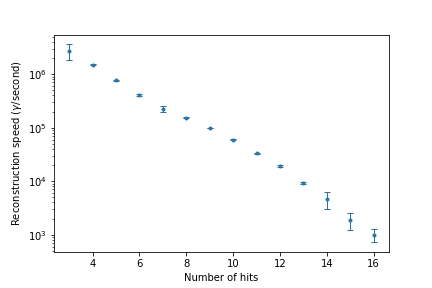
\includegraphics[width=0.7\textwidth]{graphs/pi_hits_speed.png}
    \caption{Caption}
    \label{fig:my_label}
\end{figure}

\begin{figure}
    \centering
    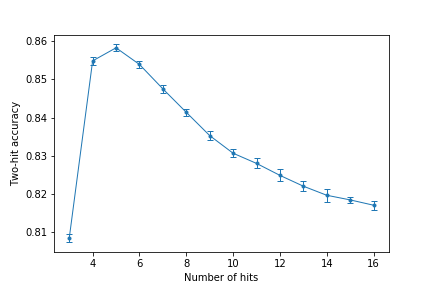
\includegraphics[width=0.7\textwidth]{graphs/pi_hits_acc.png}
    \caption{Caption}
    \label{fig:my_label}
\end{figure}

%%% Hits v hits Used

\section{Hits used in reconstruction}
- Accuracy seems to tail off around 6-8 hits for the toy model
- photons/sec goes down pretty linearly as we increase hits used
- We will likely see similar trends with Geant/real data, meaning we can fix a maximum number of hits to use (say, 10), and only sacrifice a few percentage points in accuracy while saving a significant amount of time on events with more hits.
- We expect that events with high numbers of hits will be much less likely than events with low numbers of hits, so there may be different optimal cutoffs for different source distributions.
- *** needs to be run again on the pi

\begin{figure}
    \centering
    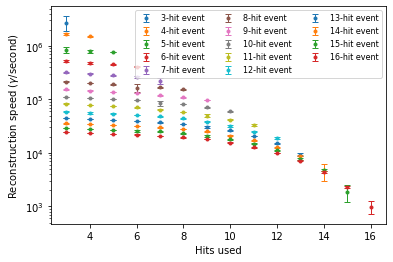
\includegraphics[width=0.7\textwidth]{graphs/pi_hits_v_hitsUsed_speed.png}
    \caption{Decrease in throughput with hits used in reconstruction}
    \label{fig:hits_v_hitsUsed}
\end{figure}

\begin{figure}
    \centering
    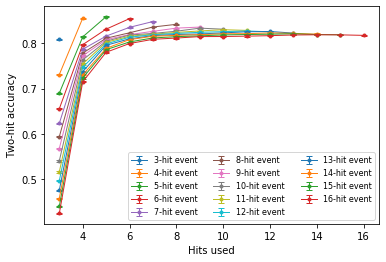
\includegraphics[width=0.7\textwidth]{graphs/pi_hits_v_hitsUsed_accuracy.png}
    \caption{Caption}
    \label{fig:my_label}
\end{figure}

\begin{figure}
    \centering
    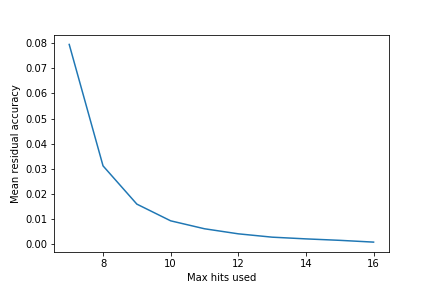
\includegraphics[width=0.7\textwidth]{graphs/mean_resid_acc.png}
    \caption{Caption}
    \label{fig:my_label}
\end{figure}

\section{p-value}
- visible correlation, but try to get a better one
- distinct downward trend in accuracy as p-value gets larger. This indicates we should use our highest p-value tested, and perhaps investigate even smaller ones.
- no clear trend in speed graph. Slight upward line until large error bar on 0.10 p-value

\begin{figure}
    \centering
    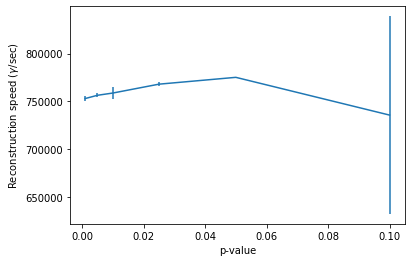
\includegraphics[width=0.7\textwidth]{graphs/pi_p_speed.png}
    \caption{Caption}
    \label{fig:my_label}
\end{figure}

\begin{figure}
    \centering
    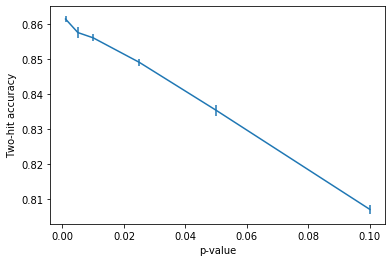
\includegraphics[width=0.7\textwidth]{graphs/pi_p_acc.png}
    \caption{Caption}
    \label{fig:my_label}
\end{figure}

\section{$\eta$-tolerance}
- There seems to be a slight periodic trend in the eta accuracy, though it is difficult to tell with the error bars
- could run with larger number of photons to find out for sure

\begin{figure}
    \centering
    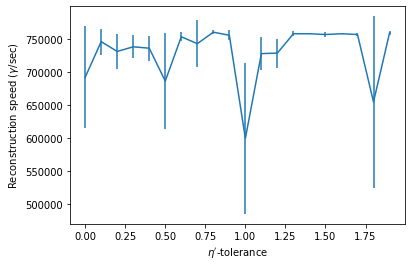
\includegraphics[width=0.7\textwidth]{graphs/pi_eta_speed.png}
    \caption{Caption}
    \label{fig:my_label}
\end{figure}

\begin{figure}
    \centering
    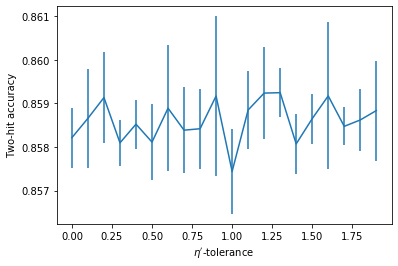
\includegraphics[width=0.7\textwidth]{graphs/pi_eta_acc.png}
    \caption{Caption}
    \label{fig:my_label}
\end{figure}

\section{Predicted Noise}
- speed for estimated energy noise has a slight downward trend, but the noise threshold is too high to draw any real conclusions. Most throughput values appear within a margin of about 10\%  of the assumed trend line.
- accuracy goes up by quite a bit when we predict more energy noise rather than less, but tails off at about 0.22, which is what the actual value of noise is. This could be incredibly useful in real-world applications, as we would be able to tell how much actual energy noise there is simply from a graph like this.
- of course, real-world applications are always more complicated, so this bears further research, but it is a promising indication.
- spatial noise does not allow us to draw many conclusions, as the ranges are so small that the error bars eclipse any minute trends in the data. 

\begin{figure}
    \centering
    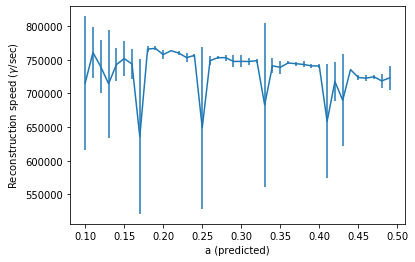
\includegraphics[width=0.7\textwidth]{graphs/pi_enFactor_speed.png}
    \caption{Caption}
    \label{fig:my_label}
\end{figure}

\begin{figure}
    \centering
    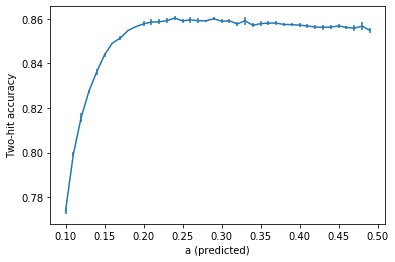
\includegraphics[width=0.7\textwidth]{graphs/pi_enFactor_acc.png}
    \caption{Caption}
    \label{fig:my_label}
\end{figure}

\begin{figure}
    \centering
    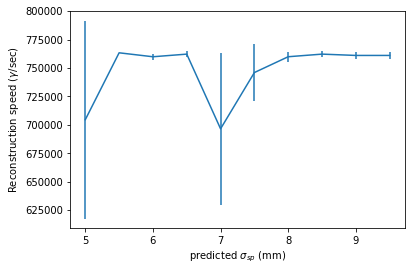
\includegraphics[width=0.7\textwidth]{graphs/pi_spFactor_speed.png}
    \caption{Caption}
    \label{fig:my_label}
\end{figure}

\begin{figure}
    \centering
    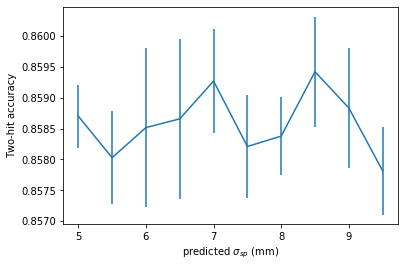
\includegraphics[width=0.7\textwidth]{graphs/pi_spFactor_acc.png}
    \caption{Caption}
    \label{fig:my_label}
\end{figure}

\section{Simulated Noise}
- helps with proof of concept - we want to check the trends are as we expect
- we expect accuracy to go down with increased noise, and it does for both
- we expect throughput to remain about the same, which it also does within some margin of error

\begin{figure}
    \centering
    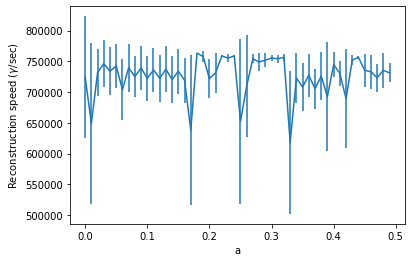
\includegraphics[width=0.7\textwidth]{graphs/pi_enNoise_speed.png}
    \caption{Caption}
    \label{fig:my_label}
\end{figure}

\begin{figure}
    \centering
    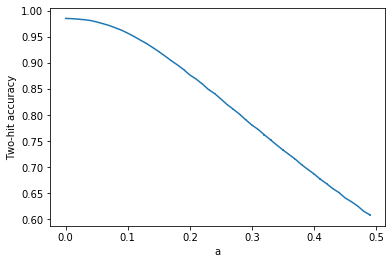
\includegraphics[width=0.7\textwidth]{graphs/pi_enNoise_acc.png}
    \caption{Caption}
    \label{fig:my_label}
\end{figure}

\begin{figure}
    \centering
    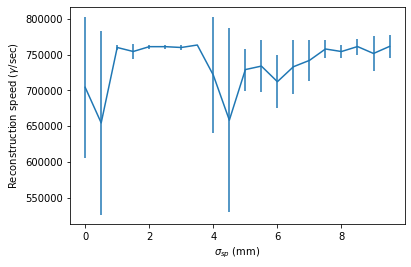
\includegraphics[width=0.7\textwidth]{graphs/pi_spNoise_speed.png}
    \caption{Caption}
    \label{fig:my_label}
\end{figure}

\begin{figure}
    \centering
    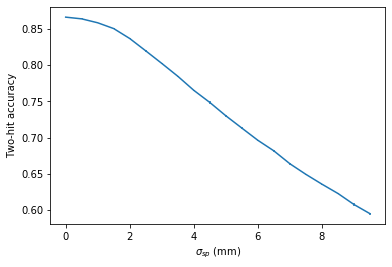
\includegraphics[width=0.7\textwidth]{graphs/pi_spNoise_acc.png}
    \caption{Caption}
    \label{fig:my_label}
\end{figure}

